\documentclass{beamer}
\usetheme{Boadilla}
\usecolortheme{sidebartab}
\beamertemplatenavigationsymbolsempty
\setbeamertemplate{footline}[frame number]
\usepackage{hyperref} 
\usepackage{graphicx}
\usepackage{color}
\usepackage{booktabs}
\usepackage{listings}
\usepackage{soul}
\usepackage{tikz}
\usepackage[utf8]{inputenc}

\definecolor{gray}{rgb}{0.4,0.4,0.4}
\definecolor{darkblue}{rgb}{0.0,0.0,0.6}
\definecolor{cyan}{rgb}{0.0,0.6,0.6}

\lstset{
	basicstyle=\ttfamily,
	columns=fullflexible,
	showstringspaces=false,
	commentstyle=\color{gray}\upshape
}

\lstdefinelanguage{XML}
{
	morestring=[b]",
	morestring=[s]{>}{<},
	morecomment=[s]{<?}{?>},
	stringstyle=\color{black},
	identifierstyle=\color{darkblue},
	keywordstyle=\color{cyan},
	morekeywords={xmlns,version,type}% list your attributes here
}

\makeatletter
\newcommand\SoulColor{%
	\let\set@color\beamerorig@set@color
	\let\reset@color\beamerorig@reset@color}
\makeatother

\lstset{language=XML}

\title{XPath}
\author{Markus Stocker}
\date{19. März 2018}

\begin{document}

\maketitle

\begin{frame}{Rekapitulation}
	
	\begin{itemize}
		\item Wie kommt es, dass ein XML Dokument eine Baumstruktur hat?
		\item Warum ist die Festlegung auf ein gemeinsames Vokabular wichtig?
		\item Wie unterstützen Programmiersprachen die Verarbeitung von XML?
		\item Was bedeutet Wohlgeformtheit?
	\end{itemize}
	
\end{frame}

\begin{frame}{Übersicht}
	
	\begin{itemize}
		\item Was is XPath
		\item XPath Konzepte
		\item Beispiele
	\end{itemize}
	
\end{frame}

\begin{frame}{What is XPath}
	
	\begin{itemize}
		\item Mit XML kann man Daten strukturieren
		\item Man kann diese in Mensch- und Maschinenlesbarer form speichern
		\item Nicht nur in Dateien sondern auch in Datenbanken
		\item Toll, aber letztlich muss man diese Daten flexibel verarbeiten können
		\item Dafür immer Programme zu schreiben ist mühsam
		\item Man benötigt Verarbeitungssprachen
	\end{itemize}
	
\end{frame}

\begin{frame}{What is XPath}
	
	\begin{itemize}
		\item Sprache zur Verarbeitung von XML Dokumenten
		\item Auf Teile eines XML Dokumentes zugreifen
		\item Navigation durch Elemente und Attribute
		\item Selektion von Elementen und Inhalten
		\item Einfache Operationen auf Inhalten
	\end{itemize}
	
\end{frame}

\begin{frame}{Knoten (\emph{node})}
	
	\begin{itemize}
		\item XPath modelliert ein XML Dokument als Knotenbaum
		\item Es gibt 7 Knotenarten
		\begin{itemize}
			\item \emph{Root node}, der virtuelle Elternknoten von \texttt{<planets>} (Wurzelelement)
			\item \emph{Element node}, z.B. \texttt{<planet>}
			\item \emph{Attribute node}, z.B. \texttt{radius="6371"}
			\item \emph{Text node}, \texttt{CDATA}
			\item \emph{Namespace node}
			\item \emph{Comment node}
			\item \emph{Processing instruction node}
		\end{itemize}
		\item Davon sind \texttt{element}, \texttt{attribute}, \texttt{text} die drei wichtigstens
	\end{itemize}
	
\end{frame}

\begin{frame}{Achsen (\emph{axis})}
	
	\begin{itemize}
		\item Navigation mittels XPath erfolgt von einem Kontextknoten
		\item Achsen bezeichnen Verwandtschaftsverhältnisse zum Kontextknoten
		\item Dreizehn unterschiedlichen Achsen
	\end{itemize}
	
\end{frame}

\begin{frame}{Achsen: Die Wichtigsten im Überblick}
	
	\begin{itemize}
		\item \emph{self}: Kontextknoten selbst
		\item \emph{child}: Kindelemente des Kontextknotens
		\item \emph{parent}: Elternelement des Kontextknotens
		\item \emph{preceding-sibling}: Vorgängige Geschwister des Kontextknotens
		\item \emph{following-sibling}: Nachfolgende Geschwister des Kontextknotens
		\item \emph{anchestor}: Vorfahren des Kontextknotens
		\item \emph{descendant}: Nachkommen des Kontextknotens
	\end{itemize}
	
\end{frame}

\begin{frame}[fragile]{Achsen: \emph{self}, der Kontextknoten}
	
	\centering
	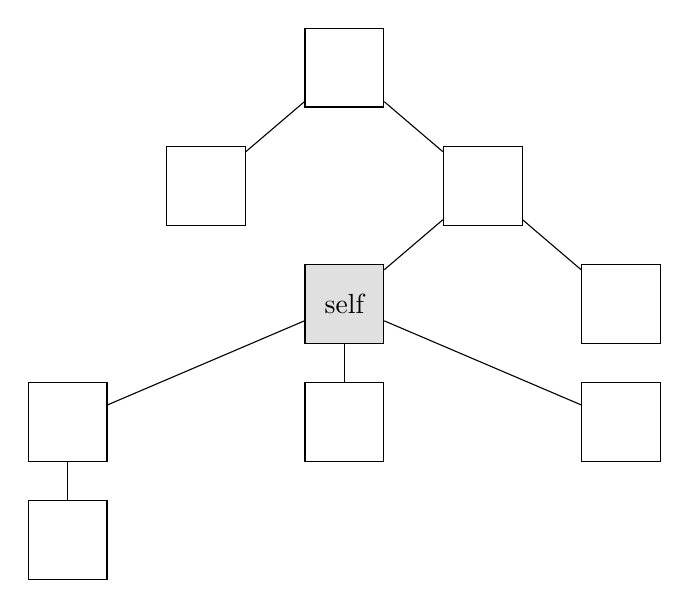
\begin{tikzpicture}[sibling distance=10em, node/.style = {shape=rectangle, draw, align=center, fill=white, minimum height=10mm, minimum width=10mm}, selected/.style = {shape=rectangle, draw, align=center, fill=gray!20, minimum height=10mm, minimum width= 10mm}]
	\node[node]{}
	child { node[node]{} }
	child { node[node]{}
		child { node[selected]{self}
			child { node[node]{} child { node[node]{} } }
			child { node[node]{} }
			child { node[node]{} } }
		child { node[node]{} } };
	\end{tikzpicture}
	
\end{frame}

\begin{frame}[fragile]{Achsen: \emph{child}, die Kinder}
	
	\centering
	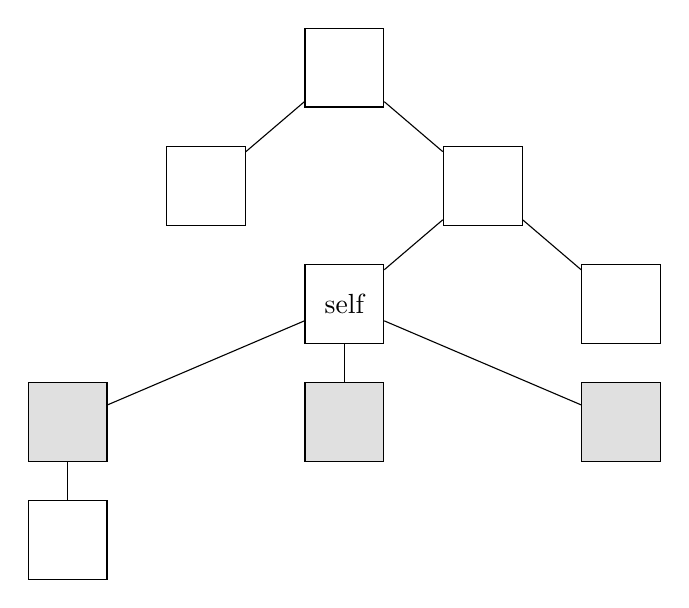
\begin{tikzpicture}[sibling distance=10em, node/.style = {shape=rectangle, draw, align=center, fill=white, minimum height=10mm, minimum width=10mm}, selected/.style = {shape=rectangle, draw, align=center, fill=gray!20, minimum height=10mm, minimum width= 10mm}]
	\node[node]{}
	child { node[node]{} }
	child { node[node]{}
		child { node[node]{self}
			child { node[selected]{} child { node[node]{} } }
			child { node[selected]{} }
			child { node[selected]{} } }
		child { node[node]{} } };
	\end{tikzpicture}
	
\end{frame}

\begin{frame}[fragile]{Achsen: \emph{parent}, das Elternteil}
	
	\centering
	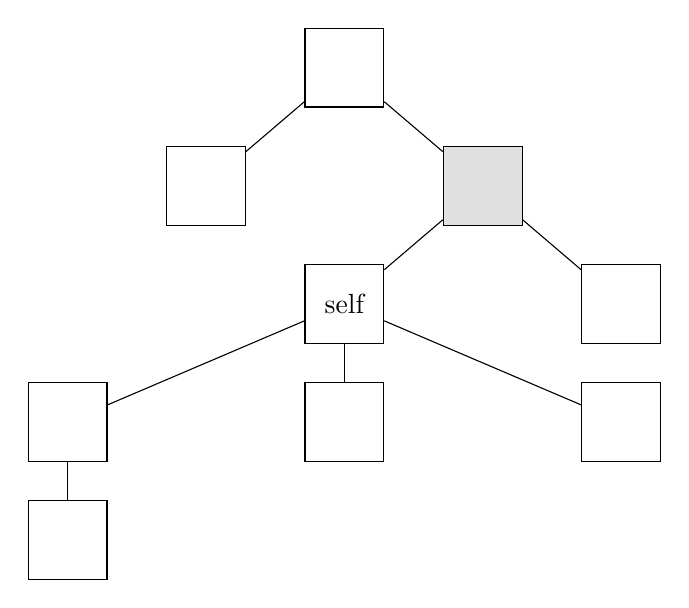
\begin{tikzpicture}[sibling distance=10em, node/.style = {shape=rectangle, draw, align=center, fill=white, minimum height=10mm, minimum width=10mm}, selected/.style = {shape=rectangle, draw, align=center, fill=gray!20, minimum height=10mm, minimum width= 10mm}]
	\node[node]{}
	child { node[node]{} }
	child { node[selected]{}
		child { node[node]{self}
			child { node[node]{} child { node[node]{} } }
			child { node[node]{} }
			child { node[node]{} } }
		child { node[node]{} } };
	\end{tikzpicture}
	
\end{frame}

\begin{frame}[fragile]{Achsen: \emph{following-sibling}, die nachfolgende Geschwister}
	
	\centering	
	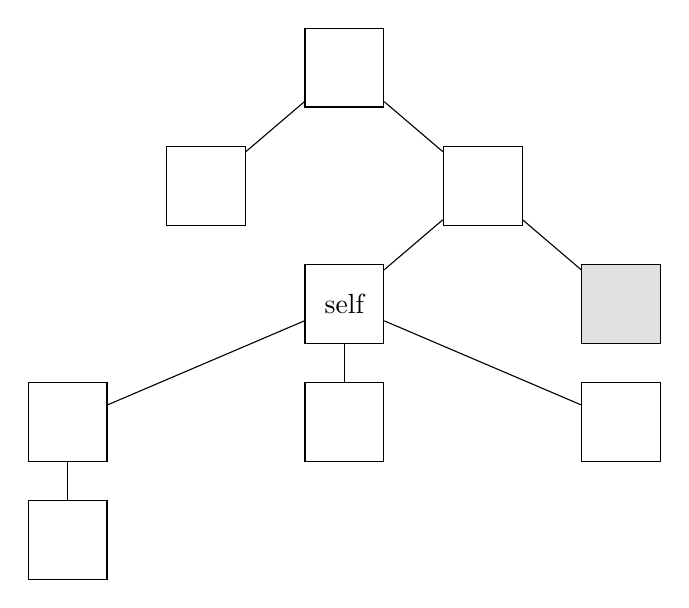
\begin{tikzpicture}[sibling distance=10em, node/.style = {shape=rectangle, draw, align=center, fill=white, minimum height=10mm, minimum width=10mm}, selected/.style = {shape=rectangle, draw, align=center, fill=gray!20, minimum height=10mm, minimum width= 10mm}]
	\node[node]{}
	child { node[node]{} }
	child { node[node]{}
		child { node[node]{self}
			child { node[node]{} child { node[node]{} } }
			child { node[node]{} }
			child { node[node]{} } }
		child { node[selected]{} } };
	\end{tikzpicture}
	
\end{frame}

\begin{frame}[fragile]{Achsen: \emph{anchestor}, die Vorfahren}
	
	\centering
	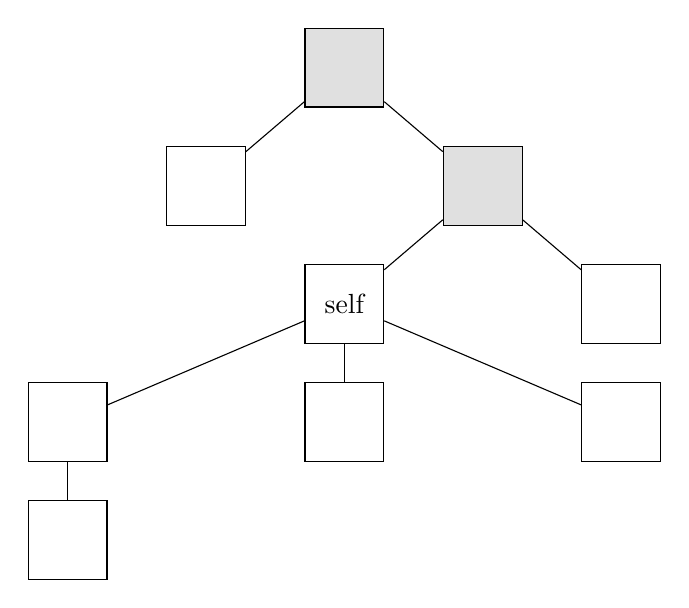
\begin{tikzpicture}[sibling distance=10em, node/.style = {shape=rectangle, draw, align=center, fill=white, minimum height=10mm, minimum width=10mm}, selected/.style = {shape=rectangle, draw, align=center, fill=gray!20, minimum height=10mm, minimum width= 10mm}]
	\node[selected]{}
	child { node[node]{} }
	child { node[selected]{}
		child { node[node]{self}
			child { node[node]{} child { node[node]{} } }
			child { node[node]{} }
			child { node[node]{} } }
		child { node[node]{} } };
	\end{tikzpicture}
	
\end{frame}

\begin{frame}[fragile]{Achsen: \emph{descendant}, die Nachkommen}
	
	\centering
	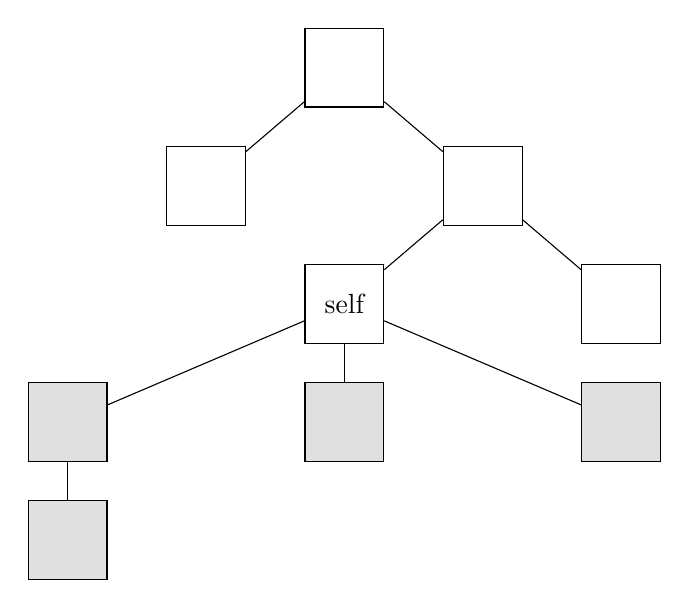
\begin{tikzpicture}[sibling distance=10em, node/.style = {shape=rectangle, draw, align=center, fill=white, minimum height=10mm, minimum width=10mm}, selected/.style = {shape=rectangle, draw, align=center, fill=gray!20, minimum height=10mm, minimum width=10mm}]
	\node[node]{}
	child { node[node]{} }
	child { node[node]{}
		child { node[node]{self}
			child { node[selected]{} child { node[selected]{} } }
			child { node[selected]{} }
			child { node[selected]{} } }
		child { node[node]{} } };
	\end{tikzpicture}
	
\end{frame}

\begin{frame}{Lokalisierungspfade}
	
	\begin{itemize}
		\item Ermöglichen die Adressierung von Knoten oder Knotenmengen	
		\item Setzen sich aus mehreren Einzelschritten zusammen
		\item Diese werden durch Schrägstriche (\texttt{/}) voneinander getrennt
	\end{itemize}
	
\end{frame}

\begin{frame}[fragile]{Lokalisierungspfade: Schritt (\emph{location step})}
	
	\begin{itemize}
		\item Bestandteile eines Schrittes
		\begin{itemize}
			\item Achse: Richtung in die aus dem Kontextknoten navigiert wird
			\item Knotentest: Der gewünschte Knoten
			\item Prädikat: Null, eins oder mehrere Filterbedingungen
		\end{itemize}
		
		\vspace{1cm}
		\centering
		\begin{verbatim}
        Achse::Knotentest[Prädikat]*
		\end{verbatim}
	\end{itemize}
	
\end{frame}

\begin{frame}[fragile]{Schritt: Beispiele}
	
	\lstset{language=XML}
	\begin{lstlisting}	
  <planets>
    <planet>
      <name radius="6371">Earth</name>
    </planet>
  </planets>
	
  child::planets
  descendant::planet[name="Earth"]
  descendant::*
	
	\end{lstlisting}
	
\end{frame}

\begin{frame}{Lokalisierungspfade}
	
	\begin{itemize}
		\item Kommen in ausführlicher oder verkürzter Form vor 
		\item Sie können relativ oder absolut sein
	\end{itemize}
	
\end{frame}

\begin{frame}[fragile]{Ausführliche und verkürzte Formen: Beispiele}
	
	\centering
	\begin{tabular}{l|l}
		\hline
		Ausführliche Form & Verkürzte Form \\
		\hline
		\texttt{child::} & \emph{Unterlassen} \\
		\texttt{attribute::} & \texttt{@} \\
		\texttt{descendant-or-self::node()/} & \texttt{//} \\
		\texttt{self::node()} & \texttt{.} \\
		\texttt{parent::node()} & \texttt{..}  \\
		\hline
	\end{tabular}
	
\end{frame}

\begin{frame}[fragile]{Absolute Lokalisierungspfade}
	
	\begin{itemize}
		\item Ausgehend vom Wurzelknoten (nicht Wurzelelement)
		\item Der erste Schrägstrich referenziert den Wurzelknoten
		\item Ermöglicht auch die Adressierung von, z.B. Kommentare
	\end{itemize}
		
	\lstset{language=XML}
	\begin{lstlisting}	
  <planets>
    <planet>
      <name>Earth</name>
      <radius>6371</radius>
    </planet>
  </planets>

  /child::planets/child::planet/child::name
  /planets/planet/name
	\end{lstlisting}
	
\end{frame}

\begin{frame}[fragile]{Relative Lokalisierungspfade}
	
	\begin{itemize}
		\item Relative Pfade benötigen einen Kontextknoten
		\item Der Pfad wird relativ zu diesem Knoten ausgewertet
	\end{itemize}
	
	\lstset{language=XML}
	\begin{lstlisting}	
  <planets>
    <planet>
      <name>Earth</name>
      <radius>6371</radius>
    </planet>
  </planets>

  child::planet/child::name
  planet/name
	\end{lstlisting}
	
\end{frame}

\begin{frame}[fragile]{Adressierung verschiedener Knotentypen}
	
	\centering
	\begin{tabular}{l|l}
		\texttt{planet/name/text()} & Textknoten des Elements \texttt{name} \\
		\texttt{planet/node()} & Alle Knotentypen (ausser Attribute) \\
		\texttt{planet/comment()} & Kommentarknoten des Elements \texttt{planet} \\
	\end{tabular}
	
\end{frame}

\begin{frame}{Prädikate}
	
	\begin{itemize}
		\item XPath Ergebnisse filtern
		\item Ermöglicht komplexere Problemstellungen
		\item Indem eine genauere Zielmenge definiert werden kann
		\item Ausdrücke die einen booleschen Wert liefern
		\item Also, wahr oder falsch
		\item Resultierende Knoten müssen auf Prädikate mit \emph{wahr} testen
		\item XPath Ausdruck liefert eine Knotenmenge 
		\item Diese wird mittels Prädikat Tests nochmals eingeschränkt
	\end{itemize}
	
\end{frame}

\begin{frame}[fragile]{Prädikate: Beispiel}
	
	\lstset{language=XML}
	\begin{lstlisting}
	
  <planets>
    <planet>
      <name radius="6371">Earth</name>
    </planet>
    <planet>
      <name>Mars</name>
    </planet>
  </planets>

  /planets/planet/name[@radius]
  /planets/planet/name[@radius = "6371"]
  planet/name[@radius = 6371]
  planet/name[@radius="6371"]/text()
  planet[name]
	\end{lstlisting}
	
\end{frame}

\begin{frame}[fragile]{Prädikate: Boolsche Operatoren}
	
	\begin{itemize}
		\item Prädikate können boolsche Operatoren enthalten
		\item Insbesondere die Operatoren \texttt{and} und \texttt{or}
	\end{itemize}
	
	\lstset{language=XML}
	\begin{lstlisting}
  <planet>
    <name radius="6371" temperature="14.9">Earth</name>
  </planet>
		
  planet/name[@radius and @temperature]
  planet/name[@radius=6371 and @temperature=14.9]
		\end{lstlisting}
	
\end{frame}

\begin{frame}[fragile]{Prädikate: Boolsche Operatoren}
	
	\lstset{language=XML}
	\begin{lstlisting}
  <planets>
    <planet>
      <name radius="6371" temperature="14.9">Earth</name>
    </planet>
    <planet>
      <name radius="3389">Mars</name>
    </planet>
  </planets>
	
  planet/name[@radius=3389 and @temperature=14.9]
  planet/name[@radius=3389 or @temperature=14.9]
	\end{lstlisting}
	
\end{frame}

\begin{frame}[fragile]{Kaskadierende Prädikate}
	
	\begin{itemize}
		\item Hintereinanderschaltung von Filtern
		\item Eine Knotenmenge wird gefiltert
		\item Es resultiert ein Ergebnis
		\item Dieses ist Ausgangsmente für das nächste Prädikat
	\end{itemize}
	
	\lstset{language=XML}
	\begin{lstlisting}
  <planet>
    <name>Earth</name>
    <radius>6371</radius>
    <temperature>14.9</temperature>
  </planet>
	
  /planet[name="Earth"][radius=6371]
	\end{lstlisting}

\end{frame}
	
\begin{frame}[fragile]{Vereinigungsmengen: Mehrere Knotentests}
	
	\lstset{language=XML}
	\begin{lstlisting}
  <planets>
    <planet>
      <name>Earth</name>
      <radius>6371</radius>
    </planet>
    <planet>
      <name radius="3389">Mars</name>
    </planet>
  </planets>
	
  planet[name="Earth"] | planet/name[@radius=3389]
	\end{lstlisting}
	
\end{frame}

\begin{frame}{Funktionen}
	
	\begin{itemize}
		\item Erweiterte Operationen und Abfragen auf Knotentests
		\item Stringanalyse von Textknoten und Attributwerten
		\item Verwendung in XPath-Ausdrücken oder Prädikaten
		\item Funktionen können ein Argument erhalten
		\item Geben immer einen Wert zurück
	\end{itemize}
	
\end{frame}

\begin{frame}[fragile]{Funktionen: Beispiele}
	
	\lstset{language=XML}
	\begin{lstlisting}
  <planets>
    <planet>
      <name>Earth</name>
      <radius>6371</radius>
    </planet>
    <planet>
      <name radius="3389">Mars</name>
    </planet>
  </planets>
	
  planet[position()=2] (oder auch planet[2])
  planet[starts-with(name, 'E')]/radius/text()
  planet[not(radius)]/name/text()
  count(planet)
  planet[last()]
	\end{lstlisting}
	
\end{frame}

\begin{frame}{Zusammenfassung}
	
	\begin{itemize}
		\item
	\end{itemize}
	
\end{frame}

\end{document}